\section{Trasduttori di deformazione - estensimetri}
Un estensimetro consente di misurare le deformazioni di un oggetto,
di conseguenza può essere usato per misurare una forza applicata, una
coppia o una pressione.
Un estensimetro è costituito da un conduttore metallico filiforme,
sottile, disposto a serpentina su una superficie di supporto. La
superficie di supporto può essere in carta alla nitrocellulosa, in
resina epossidica, fibra di vetro.

%\begin{figure}[htbp]
%	\centering
%	\includegraphics[scale=0.5]
%			{img/estensimetro.png}
%	\caption{Estensimetro\label{fig:estensimetro}}
%\end{figure}

Il supporto viene incollato all'oggetto di cui si vuole misurare la
deformazione. La sensibilità è espressa tramite il gage-factor $g$
cioè come il rapporto fra la variazione relativa della resistenza e la
variazione relativa della lunghezza:

	\[g=\frac{\frac{\Delta R}{R}}{\frac{\Delta L}{L}}\]

Si osserva che il valore della resistenza varia quando questa è
deformata secondo la legge:

	\[R=\rho\frac{L}{S} \Rightarrow L =\frac{RS}{\rho}\]

dove con $\rho$ indichiamo la resistività, con $L$ la lunghezza del
resistore e con $S$ la sua sezione.
Il conduttore filiforme è disposto a serpentina di modo da essere
molto sensibile alle deformazioni nella direzione della serpentina e
poco sensibile altrimenti. Per effetto della deformazione otteniamo:

	\[dR=\rho\frac{dL}{S} + d\rho\frac{L}{S} -
	     \rho\frac{L}{S^2}dS\]

da cui:

	\[g=\frac{LdR}{RdL}=\frac{\rho L}{SR}+
			    \frac{L^2}{SR}\frac{d\rho}{dL}-
			    \frac{L^2\rho}{S^2dLR}dS
	   =1+\frac{Ld\rho}{\rho dL} - \frac{L dS}{S dL}\]

Ricordando che un materiale sotto sforzo non modifica il proprio
volume

%FIXME altri conti che non sono chiari

%FIXME cos'era sta roba?
%La temperatura può essere influente sul valore della resistenza così
%per compensare questo disturbo si utilizzano due estensimetri con
%lavoro opposto: uno misura l'estensione, l'altro la compressione. Per
%misurare ora il valore della tensione associato alla deformazione
%utilizziamo il partitore di tensione fra i due estensimetri le cui
%resistenze valgono:

%Dove $R_1$ è per l'estensione, $R_2$ per la compressione, $R_0$
%valore a riposo della resistenza e ∆R(t) la variazione dovuta alla
%temperatura.

Gli estensimetri possono essere utilizzati anche per misurare la forza
conoscendo la deformazione di un pezzo campione, dal modulo di
elasticità e dalla sezione trasversale del provino; si può anche
misurare la coppia rilevando la deformazione di un albero mediante due
estensimetri messi a croce con inclinazione a 45° rispetto all'albero,
in questo modo un estensimetro risulta compresso e uno esteso; infine
si possono utilizzare per misurare la pressione, ma in questo caso si
utilizzano estensimetri a forma di fiore di modo che possano misurare
in ogni direzione.

\section{Trasduttori di pressione}
I più comuni sono costituiti da una membrana e da diaframmi i quali
subiscono una deformazione per effetto della pressione applicata, si
andrà poi a misurare questa deformazione con un estensimetro e quindi
convertita in grandezza elettrica. Altri tipi utilizzati sono quelli a
soffietto o a tubo di Bourdon.

\begin{figure}[htbp]
	\centering
	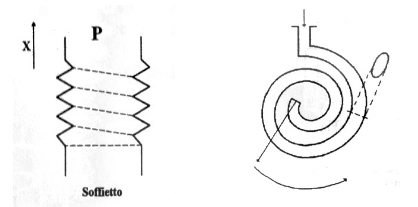
\includegraphics[scale=0.5]
			{img/pressione.png}
	\caption{Trasduttori di pressione
\label{fig:pressione}}
\end{figure}

Con il soffietto si misurano gli spostamenti, quindi si utilizzerà un
trasduttore di posizione per rilevare la pressione; il tubo di Bourdon
è costituito da un tubo a sezione ellittica avvolto a spirale alla cui
estremità è attaccato un ago: applicando la pressione sulla parte
esterna genera una rotazione dell'ago proporzionale alla pressione
imposta, andremo quindi a misurare un angolo.
I trasduttori a membrana sono utilizzati per le misure grandi, i due
tipi appena descritti, invece, per le piccole misurazioni.
\section{Trasduttori di livello - livellometri}